% !TEX TS-program = xelatex
% !TEX encoding = UTF-8 Unicode
% !Mode:: "TeX:UTF-8"

\documentclass{resume}
\usepackage{zh_CN-Adobefonts_external} % Simplified Chinese Support using external fonts (./fonts/zh_CN-Adobe/)
%\usepackage{zh_CN-Adobefonts_internal} % Simplified Chinese Support using system fonts
\usepackage{linespacing_fix} % disable extra space before next section
\usepackage{cite}
\usepackage{graphicx}


\begin{document}
\pagestyle{empty} % 移除页码

% ---------------heading------------------

% 图右文左
\begin{minipage}[c]{0.85\textwidth} % 信息部分
  \leftInfo{袁浩}{(+86) 198-2277-7378}{sirius1y@outlook.com}{http://sirius1y.top/}{sirius2alpha}
\end{minipage}
\begin{minipage}[c]{0.13\textwidth} % 照片部分,居中对齐
  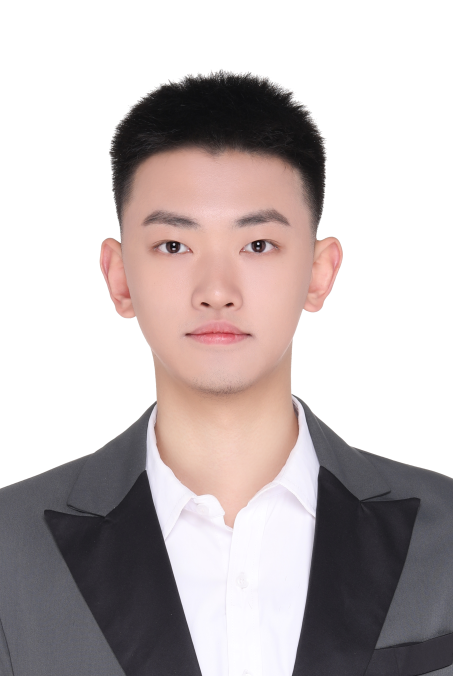
\includegraphics[width=\textwidth]{photo.png}
\end{minipage}

% 图左文右
% \begin{minipage}[c]{0.14\textwidth} % 照片部分,居中对齐
%   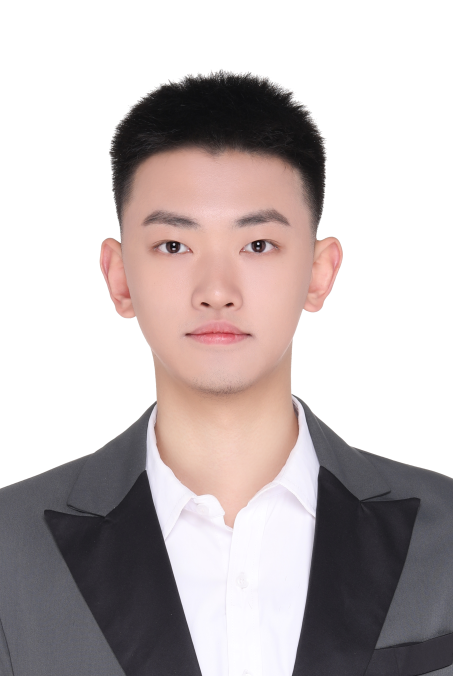
\includegraphics[width=\textwidth]{photo.png}
% \end{minipage}
% \hspace*{\fill}
% \begin{minipage}[c]{0.85\textwidth} % 信息部分
%   \rightInfo{袁浩}{(+86) 198-2277-7378}{sirius1y@outlook.com}{http://sirius1y.top/}{sirius2alpha}
% \end{minipage}
% \vspace{1ex}

% 带照片的排版,左右对齐
% \begin{minipage}[c]{0.12\textwidth} % 照片部分,居中对齐
%   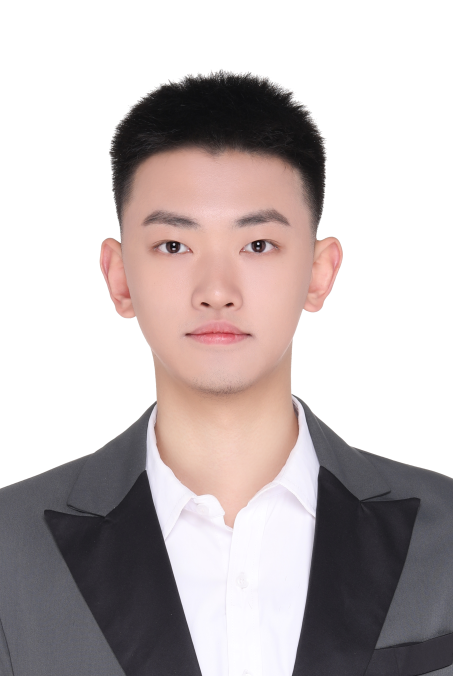
\includegraphics[width=\textwidth]{photo.png}
% \end{minipage}
% \hfill
% \begin{minipage}[c]{0.85\textwidth} % 信息部分
%   \tableInfo{袁浩}{http://sirius1y.top/}{(+86) 198-2277-7378}{sirius1y@outlook.com}
% \end{minipage}
% \vspace{1.2ex}

% 不带照片的排版
% \name{袁浩}
% \vspace{1.2ex}
% \contactInfo{}{Phone (+86) 198-2277-7378}{E-mail sirius1y@outlook.com}{}
% \contactInfo{}{Blog http://sirius1y.top/}{GitHub @sirius2alpha}{}

% ---------------body------------------

\section{个人总结}
本人具有一定的后端开发能力,对项目的开发流程有一些了解,有多次网站设计开发的经历。乐于沟通,善于和他人共同完成项目开发,曾参加了如ASC学生超级计算机挑战赛,能够做到积极主动沟通。具有一定的适应能力,能够服从安排,做一些力所能及的事。学习能力较强,对新事物的理解学习速度快,也乐于听从前辈的指点。

% \section{\faGraduationCap\ 教育背景}
\section{教育背景}
\datedsubsection{\textbf{上海大学},计算机科学与技术,\textit{在读本科生}}{2021.09 - 2025.06}
\ \ 曾任职团支部书记,获得“活力团支部”荣誉称号

% \section{\faCogs\ IT 技能}
\section{技术能力}
% increase linespacing [parsep=0.5ex]
\begin{itemize}[parsep=0.5ex]
  \item \textbf{编程语言}: Go, C++, Python, Shell
  \item \textbf{计算机基础}: 熟练掌握计算机网络、数据结构和算法、操作系统
  \item \textbf{Linux}: 熟练使用Linux有两年经验,项目基本都是在Linux上进行开发和部署
  \item \textbf{工具}: 掌握Git、Docker等开发工具
  \item \textbf{数据库}: 使用过MySQL、MongoDB、Redis等数据库,搭建过Redis集群
  \item \textbf{框架}:有过Gin、Flask、Django、Vue等项目框架的开发经历
  \item \textbf{分布式}:在云服务器上部署过Kubernetes和Hadoop
\end{itemize}

% \end{itemize}

% \section{实习经历}
% \datedsubsection{\textbf{阿里巴巴集团 | Alibaba}, 前端开发工程师}{2017.6-2017.9}
% \begin{itemize}
% %   \item 飞猪北京前端团队全面负责各交通线的票务(机票/火车票/汽车票) web 应用与事业群基础架构研发
%   \item 独立负责车站地图开发(React),通过HTML5 本地存储及JSBridge实现在阿里全系应用中发布上线
%   \item 独立负责BU SPM chrome插件开发,支付成功/订单详情等页面的开发与交叉营销的接入工作
% \end{itemize}

% \datedsubsection{\textbf{北京腾云天下科技有限公司 | TalkingData},数据挖掘与可视化工程师}{2015.11-2017.5}
% \begin{itemize}
%   \item \textbf{利用海量用户定位数据,对城市空间及人群移动特征进行研究。}第一个课题是基于香农熵和人群出行模式,构建城市网格与用户矩阵分析城市多样性/流动性分布;可视分析平台前端与可视化基于D3/Vue/Express开发,数据分析与存储采用Python/MySQL/MongoDB技术,为了均衡大数据情况下的页面可视化渲染消耗用canvas替代svg。第二个课题是对海量商场定位数据做人群分类与可视化查询,依据该系统撰写的论文被CIKM 2016(DAVA Workshop)录用,并收录于中科院软件所年会成果集
%   \item 负责数据科学部HQ LAB的可视化原型开发,主导 TalkingMind 平台系统设计与前端开发
% \end{itemize}

% \datedsubsection{\textbf{北京格灵深瞳信息技术有限公司 | DeepGlint},Web开发工程师}{2015.7-2015.9}
% \begin{itemize}
%   \item \textbf{独立负责MUSE部门的可视化组件研发。}与平台研发、设计协作完成 DeepGlint Developer 平台可视化图表组件的集成开发,符合完全定制化渲染、响应式布局与实时更新等特点
%   \item 利用 D3+Vue+WebGL(Three.js) 尝试实现三维空间的人群移动可视化
% \end{itemize}

% \begin{onehalfspacing}
% \end{onehalfspacing}

% \datedsubsection{\textbf{DID-ACTE} 荷兰莱顿}{2015年3月 - 2015年6月}
% \role{本科毕业设计}{LIACS 交换生}
% 利用结巴分词对中国古文进行分词与词性标注,用已有领域知识训练形成 classifier 并对结果进行调优
% \begin{onehalfspacing}
% \begin{itemize}
%   \item 利用结巴分词对中国古文进行分词与词性标注
%   \item 利用已有领域知识训练形成 classifier, 并用分词结果进行测试反馈
%   \item 尝试不同规则,对 classifier 进行调优
% \end{itemize}
% \end{onehalfspacing}

% \section{\faHeartO\ 项目/作品摘要}
\section{项目经历}
\begin{itemize}
    \item \datedsubsection{\textbf{全国大学生市场调查与分析大赛数据分析}( \textit{http://www.china-cssc.org/} )}{2024.02}
    \ \begin{itemize}
        \item 使用Selenium库对携程评论爬虫
        \item 基于CART决策树、K-原型聚类等方法分析
    \ \end{itemize}

    \item \datedsubsection{\textbf{点击次数排行榜网站}( \textit{http://redisboard.sirius1y.top/} )}{2024.01}
    \ \begin{itemize}
      \item 全栈开发,使用Vue + Gin + Redis等技术
      \item 使用WebSocket进行前后端的持续更新
    \ \end{itemize}

    \item \datedsubsection{\textbf{部署Blog到华为云服务器}( \textit{http://sirius1y.top/} )}{2023.12}
    \ \begin{itemize}
      \item 使用Nginx作为Web服务器
    \ \end{itemize}

    \item \datedsubsection{\textbf{选课系统网站}( \textit{https://github.com/sirius2alpha/CourseSystem} )}{2023.09}
    \ \begin{itemize}
      \item 负责网站整体的设计,以及前端和API的开发
      \item 前端使用Vue框架,API设计遵循RESTful设计原则
      \item 使用Git进行团队协作
    \ \end{itemize}

  \end{itemize}

  \section{竞赛获奖}
% increase linespacing [parsep=0.5ex]
\begin{itemize}[parsep=0.2ex]
%   \item LeetCodeOJ Solutions, \textit{https://github.com/hijiangtao/LeetCodeOJ}
\item \datedsubsection{上海大学领导力奖学金}{2022.12}
\item \datedsubsection{上海大学公益爱心奖学金}{2022.12}
\item \datedsubsection{第14届全国大学生广告艺术大赛( \textit{https://sun-ada.net/} ),\textbf{上海市三等奖}}{2022.07}
\end{itemize}

% % \section{\faInfo\ 社会实践/其他}
\section{社会实践}
% increase linespacing [parsep=0.5ex]
\begin{itemize}[parsep=0.2ex]
  \item \datedsubsection{前往贵州省盘州市参与市场调研,解决乌蒙大草原景区满意度低的问题}{2024.01}
  \item \datedsubsection{前往上海市普陀区真如镇街道参与科技助老服务,上海大学“点石成金”团队}{2023.10}
\end{itemize}

%% Reference
%\newpage
%\bibliographystyle{IEEETran}
%\bibliography{mycite}
\end{document}
